\chapter{总结与展望} \label{chapter:conclusion}

\epigraph{... the ways by which men arrive at knowledge of the celestial things are hardly less wonderful than the nature of these things themselves}{\textit{Johannes Kepler}}


\section{更丰富的行星样本}

在短短二十年内,系外行星领域在仪器方面可谓发生了质的飞跃,新发现的系统也一次又一次地
打翻了以往我们对于行星陈旧的认知。可我们在系外行星这条探索之路上才刚刚启程,下一步科
学研究依旧得依赖更多与更深的挖掘。在仪器方面,传统的视向速度依然在稳步中不断提高仪器
的谱分辨率与可靠度(如 TESS\cite{Ricker2015} 与 PLATO\cite{Rauer2014})以尝试去发现更
多的中长周期行星,这包括温木星(warm Jupiter)以及更长周期的冷木星。其中对温木星的探
测与刻画是通往解释它们自身以及热木星形成的必经之路
\cite{Petrovich2016,Huang2016,Dong2014a,Frewen2016,Dawson2014a,Antonini2016}。
在目前形成热木星的机制中,盘迁移能够解释低偏心率以及处于共振的系统,偏心率较中等的系
统则往往只能通过行星---行星散射形成,而更高偏心率的则很可能正处于强烈的潮汐圆化过程。
如何区分不同的机制以及温木星究竟是不是失败的热木星,都是非常值得探究的问题。这群特殊
的木星在解开行星形成密钥的同时,也对恒星的演化有着重要的暗示,具体请见 \S \ref{sec:fateofplanets})。

再者,利用已知行星系统去寻找发现质量更小的超级行星也十分有趣。类似 WASP-47 这样的系统
在观测中又究竟还有多少遗漏,而小质量行星的信号到底会不会被掩埋在已存在巨行星的 RV 信号
中呢?这些问题必须得利用多观测手段同时查漏来解答,比如 \textit{Gaia} 卫星的天体测量数据可
用来解除拟合参数中轨道倾角 $i$ 与真实质量的简并\cite{Gaia2016},并且在探测一些处于共振的
行星系统也有独特的优势\cite{Wu2016}。

相比之下,凌星法在探测系外行星的密度,表层大气环流以及压强温度垂直分布轮廓有着独特的先
机(如图 \ref{fig:transitspectro}),直接成像法亦可直接测量行星的光谱。如今这部分系统只有三十
颗行星成功利用 \textit{Spitzer} 与 Hubble 观测到其高层大气结构和垂直温度分布,如系统 HD 189733 b
\cite{Knutson2007}。利用凌星发测得的行星半径与 RV 得到的质量还可以初步限定行星的密度(如
图 \ref{fig:massrad})。对诸多天体研究\cite{Baraffe2008,Fortney2007}显示从恒星级天体到类地行
星,质量与半径的关系呈现出截然不同的指数系数:

\begin{equation} \label{eq:massrad}
R \propto \left\{
  \begin{array}{lr}
       \,   M            &  \qquad \text{恒星} 	   \\
       \,   M^{-1/8}  &  \qquad \text{褐矮星} 	   \\
       \,   M^{1/10} &  \qquad \text{气巨行星}   \\
       \,   M^{1/3}   &  \qquad \text{类地行星} 
  \end{array}
\right.
\end{equation} \myequation{不同天体的质量半径关系}

这些关系恰恰可以反映行星内部的成分以及物态方程\cite{Zapolsky1969}。同样的,超级地球中大
气与固体组成构造的差别也将能很好的解释类似超级地球等「过渡型」行星究竟是失败的气巨星还
是大个头的地球\cite{Rogers2015a,Lissauer2014},这也能帮助我们了解超级地球在原行星盘中的
形成地点和演化吸积过程\cite{Miguel2011,Haghighipour2013}。

\begin{figure}[t]
\centering
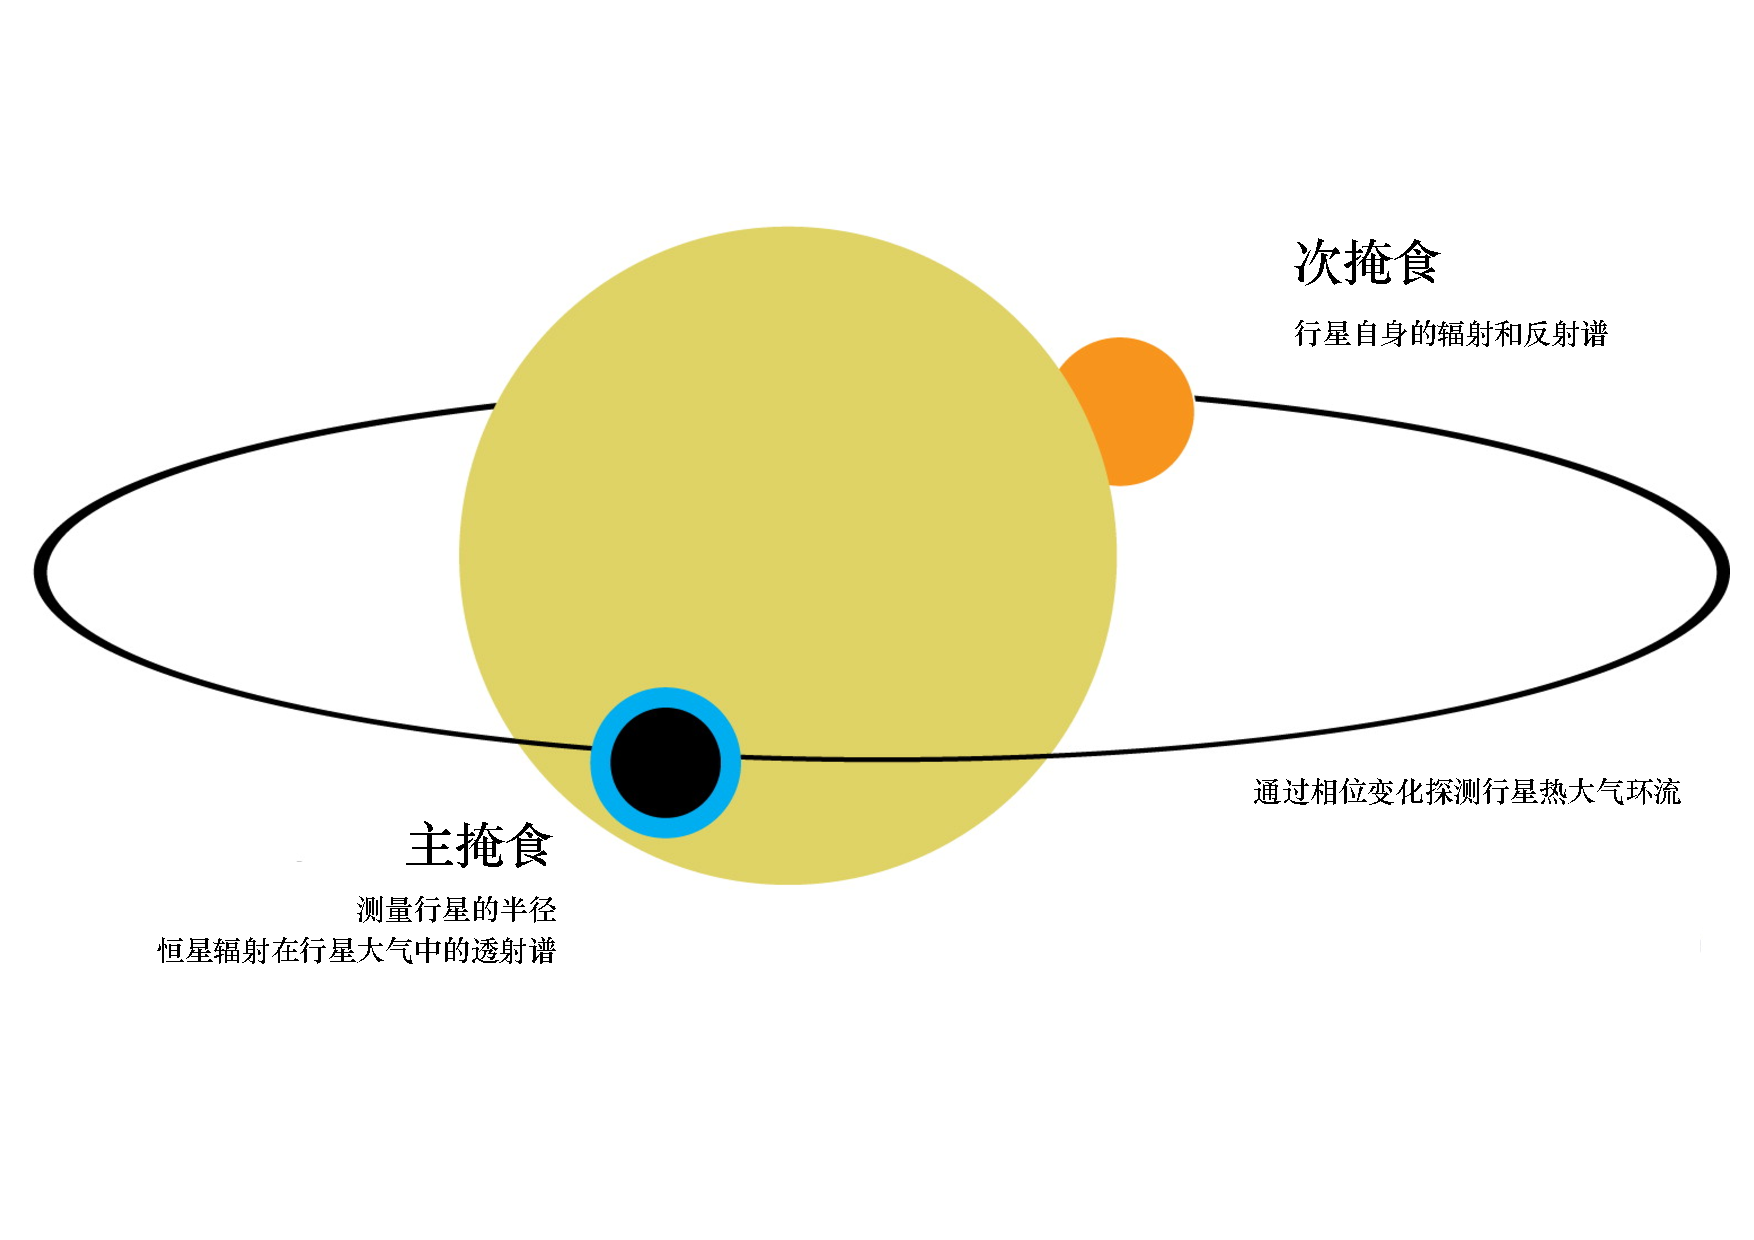
\includegraphics[width=1.0\textwidth]{figures/chapter5/fig1_eclipsing.pdf}
\caption{凌星探测法对行星物理性质的后续观测示意图。从主掩食(Transit)到次掩食(Occultation)可以分别看到行星大气随着相位变化以及行星大气所蕴含的半径和大气成分等重要信息。图片版权 Sara Seager。}
\label{fig:transitspectro}
\end{figure}


除了研究这些特殊的行星之外,另一个更重要的目标就是将行星质量探测下限延伸至类地行星甚至
系外卫星。目前系外卫星探测率至今仍为零\cite{Kipping2011},而在探测极限允许的条件下,这很
可能与主星的光致蒸发与动力学作用相关\cite{Yang2016}。探测地球质量与大小的行星对于技术而
言非常具有挑战性,比如类太阳主星的 P 模震荡以及表面米粒组织所引起的 Doppler Jitter 能直接
掩盖等同类地行星造成的 RV 振幅。正因为通往发现类太阳周围的类地行星任务非常艰巨,从而许
多未来的科学目标均广泛集中在 M 型矮星周围,甚至太阳系内更外围的第九大行星\cite{Batygin2016a}。


\begin{figure}[t]
\centering
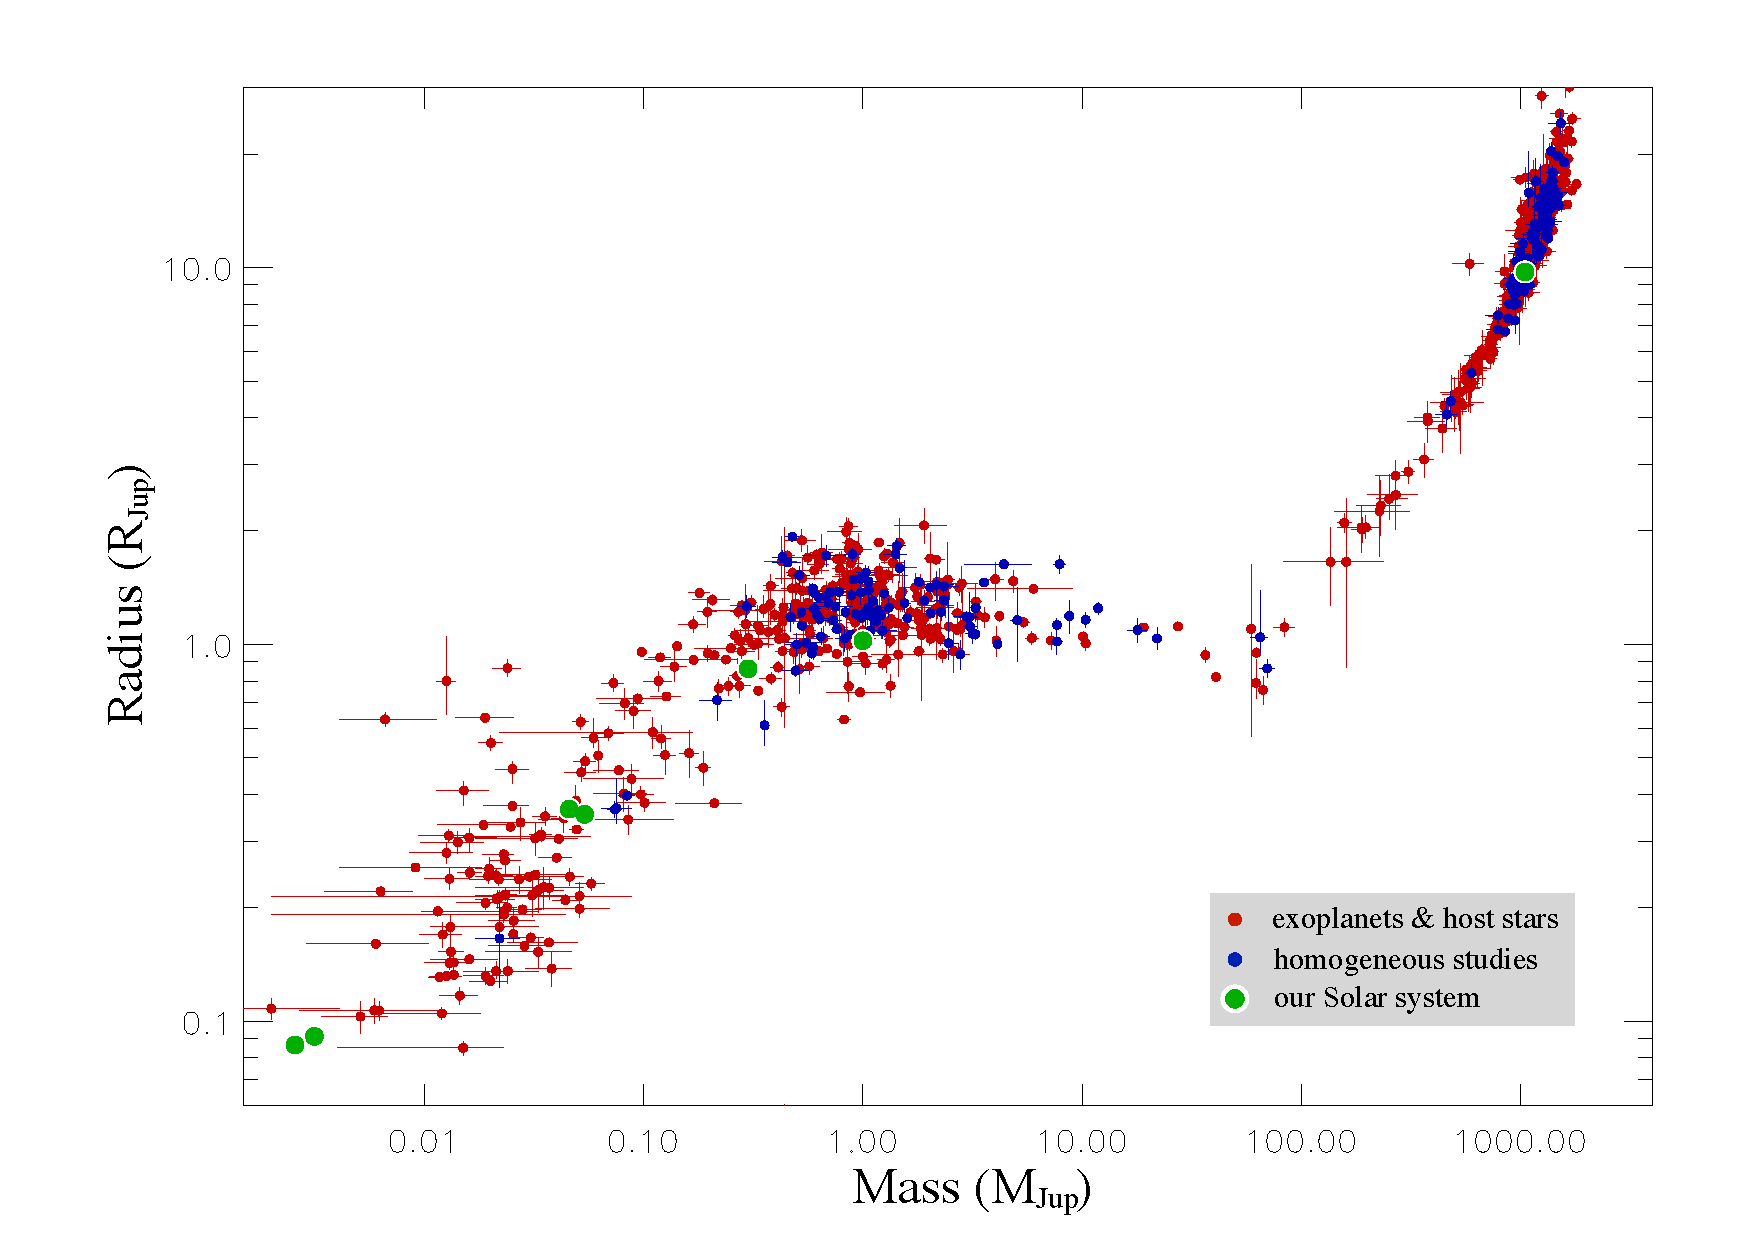
\includegraphics[width=1.0\textwidth]{figures/chapter5/fig2_massrad.pdf}
\caption{凌星法探测的行星的质量与半径关系图(包括其主星)。从恒星、矮星到气态巨行星与类地行星半径质量关系呈现处的不同变化向我们反映了它们内部结构与物质状态的不同。此图数据源自网站 TEPCat。}
\label{fig:massrad}
\end{figure}
 

\section{全局的行星系统演化} \label{sec:fateofplanets}

作为行星原材料的摇篮,恒星以及诞生恒星的分子云和周边的星际空间在支配恒星以及后续的行星
演化有着至关重要的作用。一些研究显示不同的质量以及金属丰富的主星会对其中行星出现的概率
和质量其决定性因素\cite{Fischer2005},比如 M 型矮星周围的气巨星形成率会偏低,而类地行星则
正好相反\cite{Johnson2007b,Cumming2008,Kennedy2008},而随着恒星质量的增加大质量行星出
现的概率也会偏大,比如对于巨星和亚巨星分支,这类恒星周围更容易看到大质量行星\cite{Johnson2007}。
但与此同时,巨星周围的短周期热木星出现的概率却又偏少(共 99 个系外行星处于巨星周围,其中
周期小于 10 天的却只有 2 颗\footnote{\url{https://www.lsw.uni-heidelberg.de/users/sreffert/giantplanets/giantplanets.php}})。
这很可能是因为主星半径膨胀后潮汐作用将行星吞噬后的演化结果\cite{Sato2008,LilloBox2016}。


此外,在双星或者多星系统环境中行星形成过程和对类地行星的影响也不可小觑\cite{Desidera2007}。
太阳系内木星与地球可以同时存活,可是在双星系统中(如图 \ref{fig:staraffp} 所示)情况却大有不同,
在三体不稳定模型下\cite{Marzari2007},由于混沌效应,行星产生的概率明显随着恒星的交汇次数以
及时间而减小,同样若行星系统中存在类似木星的长周期行星,那么将对内行星系统造成更强的摧毁
效应,而且散射至外围的行星也可能是环双星行星候选体的一种形成机制\cite{Gong2013}。


\begin{figure}[t!]
\centering
\begin{subfigure}[b]{.48\textwidth}
\captionsetup{width=0.9\textwidth}
\centering
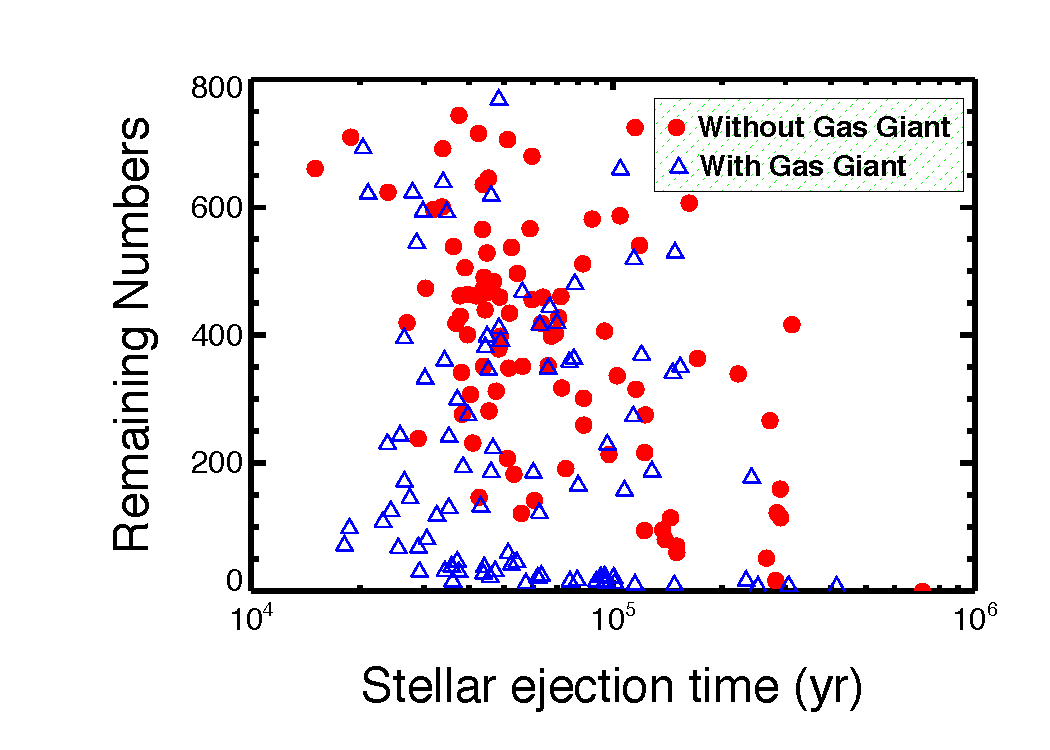
\includegraphics[width=0.95\textwidth]{figures/chapter5/fig3a_stellarenv.pdf}
\caption{恒星发生不稳定的时标对于行星系统内行星的存活率造成的影响。图中三角形表示质量为零的测试粒子(Testing Particle,TP)情况,而红色圆点则表示在系统中加入一颗木星质量的行星后木星的存活对 TPs 的影响。}
\end{subfigure}
\begin{subfigure}[b]{.48\textwidth}
\captionsetup{width=0.9\textwidth}
\centering
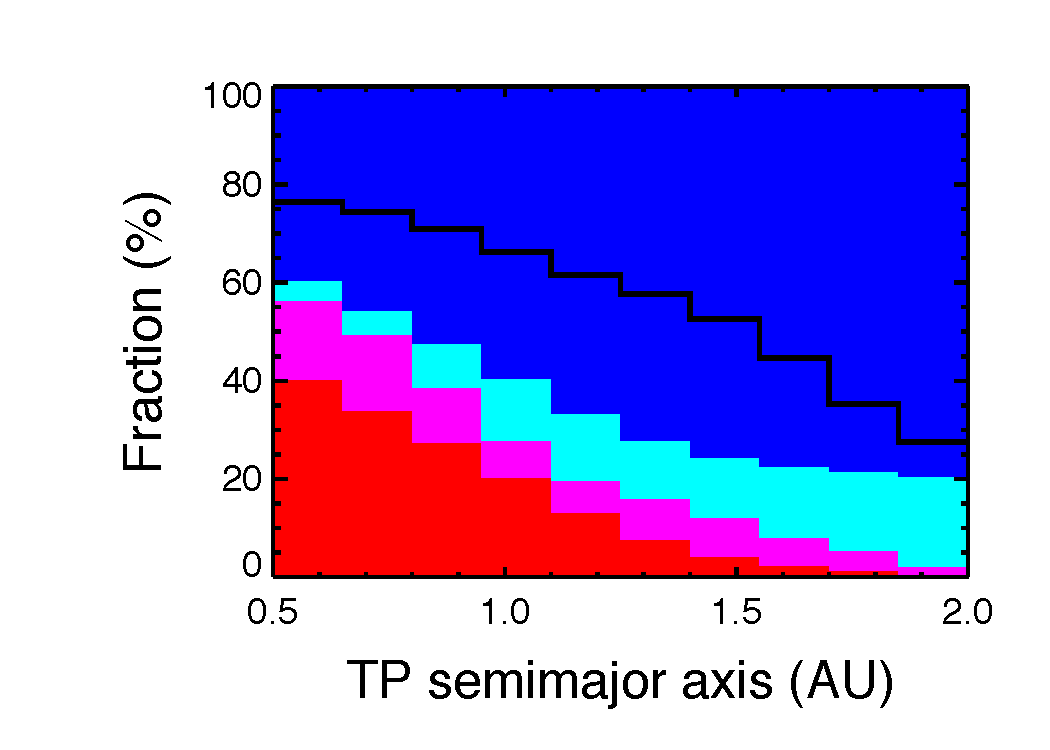
\includegraphics[width=0.95\textwidth]{figures/chapter5/fig3b_innerplanet.pdf}
\caption{在不同半长径下红色(气巨星逃逸, TPs 存活)、紫色(气巨星 TPs 均存活)、浅蓝色(气巨星存活, TPs 逃逸)与深蓝色(气巨星与 TPs 均逃逸 )的概率。黑色线则表示未添加气巨星,TPs 的存活比例。}
\end{subfigure}
\caption{恒星在多星系统中的形成环境对行星系统的影响:三星系统由于三体不稳定性会导致其中两颗恒星发生密近交汇,这种剧烈的动力学过程会导致行星系统发生不稳定性,此效应更会对恒星周围其他的行星如类地行星产生恶性连锁反应,因而气巨星对类地行星存在几乎是种灾难。}
\label{fig:staraffp} 
\end{figure}


随着恒星与行星系统的演化,灾难在所难免。比如在白矮星周围,光谱观测看到了其表面的重金属
污染\cite{Barstow2014},这样的污染很可能因为行星系统被潮汐撕裂后留下的残骸撞击中心致密性
导致的\cite{Vanderburg2015,Boyajian2016}。对于一些紧密间隔的行星系统,行星的不稳定时标大
大缩短\cite{Lissauer2011,Lovis2011,MacDonald2016},而就连太阳系内长期演化后都可能导致各大
行星之间的不稳定性发生,从而造成轨道交错以致最后彼此互相摧毁,化为碎屑\cite{Laskar1988,Laskar1990}。


\section{具现代化的范式转换}

当今的科学是一项重任,取之于民同时用之于民。全民参与以为着新的时代已经悄然到来(Citizen 
Science),其中 Zooniverse\footnote{\url{https://www.zooniverse.org}} 旗下的 Planet Hunters 已经
发表了十二篇文章,包括第一篇被认证的系外行星(参见文献 \citen{Schwamb2013} )。更多人提供
了额外能够让人们参与进来的提议,包括命名系外行星\footnote{\url{http://nameexoworlds.iau.org/}}
以及其它越来越丰富的可能性\cite{Hessman2010,Marshall2015}。在软件层面,整合源代码网站 
ASCL\footnote{\url{http://ascl.net/}} 以及越来越多建立在 Python 之上的开发工具也在极大程度上降低
了数据分析的门槛,如 Astropy \footnote{\url{http://www.astropy.org/}} 与 
Rebound\footnote{\url{https://github.com/hannorein/rebound}}。

另外利用机器学习(machine learning)分析以及深度挖掘数据(data mining)也将会在天文领域有
相应的一席之地\cite{Ball2010,McCauliff2015,Thompson2015}。若要结合大数据(big data)来反馈
到系外行星领域,星族合成方法(Population Synthesis )也许是最能够还原众多系外行星集体性质
与演化的途径之一\cite{Benz2014,Mordasini2009}。

\section{细致刻画单个系统}

随着样本的增多,统计结果越来越丰富。然而如若想清楚地知道行星是否可能存在生命,我们还得通
过研究刻画单个系统的宜居性来得出结论。在 HEC 列表
\footnote{\url{http://phl.upr.edu/projects/habitable-exoplanets-catalog}}中,总共也列出约 50 颗的潜
在宜居住行星(habitable exoplanets),那么我们究竟该如何定义宜居性\cite{Kasting1993},而宜居
性又是否与行星本身的质量、温度、大气与液态水、其他行星以及主星的活动之间(尤其是 M 型恒星)
有必然关联\cite{Kasting2003,Segura2005,Scalo2007}?其中包括对距离我们最近的行星系统 Proxima 
Centauri b 的主星、伴星、行星性质以及其间的空间天气环境对宜居性的讨论(参见 
\citen{AngladaEscude2016} 以及其引用文献)。

而为了得到更精确的行星内部结构,未来则可通过分析太阳系内气巨星以及类地行星的深层内部结构
以及 USPs 或者 HJs 来了解其它行星的性质。此外系外生命的存在信号(即系外生物信号,
biosignature)以及她们的存在是否真的依赖类似地球大气中的 O$_2$ 等等。这些问题或许都值得去
等待诸如 James Webb Space Telescope(JWST) 卫星的发射来揭晓,系外行星科学在下一个纪元
的里程碑也许就在前方的迷雾之中。









